%--------------------------------------
%ELECTROTECHNIQUE - SCHEMA DE LIAISON A LA TERRE
%--------------------------------------

%utiliser les environnement \begin{comment} \end{comment} pour mettre en commentaire le préambule une fois la programmation appelée dans le document maître (!ne pas oublier de mettre en commentaire \end{document}!)

\begin{comment}

\documentclass[a4paper, 11pt, twoside, fleqn]{memoir}

\usepackage{AOCDTF}

%--------------------------------------
%CANEVAS
%--------------------------------------

\newcommand\BoxColor{\ifcase\thechapshift blue!30\or brown!30\or pink!30\or cyan!30\or green!30\or teal!30\or purple!30\or red!30\or olive!30\or orange!30\or lime!30\or gray!\or magenta!30\else yellow!30\fi} %définition de la couleur des marqueurs de chapitre

\newcounter{chapshift} %compteur de chapitre du marqueur de chapitre
\addtocounter{chapshift}{-1}
	
\newif\ifFrame %instruction conditionnelle pour les couleurs des pages
\Frametrue

\pagestyle{plain}

% the main command; the mandatory argument sets the color of the vertical box
\newcommand\ChapFrame{%
\AddEverypageHook{%
\ifFrame
\ifthenelse{\isodd{\value{page}}}
  {\backgroundsetup{contents={%
  \begin{tikzpicture}[overlay,remember picture]
  \node[
  	rounded corners=3pt,
    fill=\BoxColor,
    inner sep=0pt,
    rectangle,
    text width=1.3cm,
    text height=5.5cm,
    align=center,
    anchor=north west
  ] 
  at ($ (current page.north west) + (-0cm,-2*\thechapshift cm) $) %nombre négatif = espacement des marqueurs entre les différents chapitres (à régler en fin de rédaction) (4.5cm vaut un espacement équivalement à la hauteur du marqueur, une page peut en contenir 6 avec cet espacement-la mais il est le plus équilibré)
    {\rotatebox{90}{\hspace*{.3cm}%
      \parbox[c][0.9cm][t]{5cm}{%
        \raggedright\textcolor{black}{\sffamily\textbf{\leftmark}}}}};
  \end{tikzpicture}}}
  }
  {\backgroundsetup{contents={%
  \begin{tikzpicture}[overlay,remember picture]
  \node[
  	rounded corners=3pt,
    fill=\BoxColor,
    inner sep=0pt,
    rectangle,
    text width=1.3cm,
    text height=5.5cm,
    align=center,
    anchor=north east
  ] 
  at ($ (current page.north east) + (-0cm,-2*\thechapshift cm) $) %nombre négatif = espacement des marqueurs entre les différents chapitres (à régler en fin de rédaction) (4.5cm vaut un espacement équivalement à la hauteur du marqueur, une page peut en contenir 6 avec cet espacement-la mais il est le plus équilibré)
    {\rotatebox{90}{\hspace*{.3cm}%
      \parbox[c][0.9cm][t]{5cm}{%
        \raggedright\textcolor{black}{\sffamily\textbf{\leftmark}}}}};
  \end{tikzpicture}}}%
  }
  \BgMaterial%
  \fi%
}%
  \stepcounter{chapshift}
}

\renewcommand\chaptermark[1]{\markboth{\thechapter.~#1}{}} %redéfinition du marqueur de chapitre pour ne contenir que le titre du chapitre %à personnaliser selon le nombre de chapitre dans le cours

%--------------------------------------
%corps du document
%--------------------------------------

\begin{document} %corps du document
	\openleft %début de chapitre à gauche

\end{comment}

\begin{figure}
\centering
\caption{Effets du courants sur le corps humain \label{fig:effets_courant_electrique}}
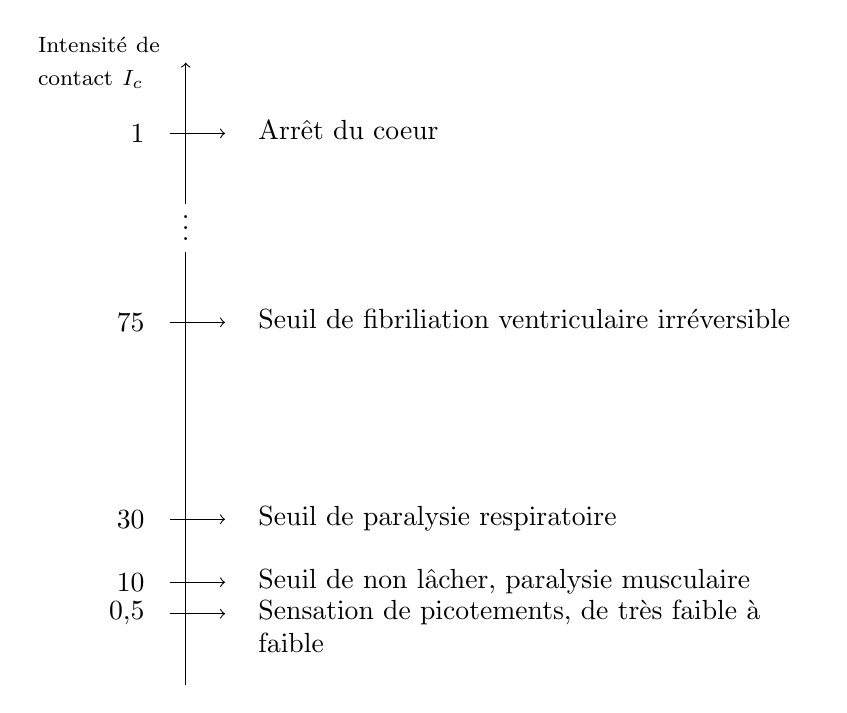
\begin{tikzpicture}
%\DrawGrid{(-7,-5)}{(7,5)} %grille d'aide pour le placement des objets

\draw (-7,4) node [right, minimum width=2cm, text width=1.8cm] {\footnotesize{Intensité de contact $I_c$}};
\draw [->] (-5,2.2) -- (-5,4);
\draw (-5, 2) node {\vdots};
\draw (-5,-3.9) -- (-5,1.6);
\draw (-5.4,-3) node [left] {\SI{0,5}{\milli\ampere}};
\draw [->] (-5.2,-3) -- (-4.5,-3);
\draw (-4.2,-3) node [anchor=mid west, text width=7cm] (A) {Sensation de picotements, de très faible à faible};
\draw (-5.4,-2.6) node [left] {\SI{10}{\milli\ampere}};
\draw [->] (-5.2,-2.6) -- (-4.5,-2.6);
\draw (-4.2,-2.6) node [anchor=mid west, text width=7cm] {Seuil de non lâcher, paralysie musculaire};
\draw (-5.4,-1.8) node [left] {\SI{30}{\milli\ampere}};
\draw [->] (-5.2,-1.8) -- (-4.5,-1.8);
\draw (-4.2,-1.8) node [anchor=mid west, text width=7cm] {Seuil de paralysie respiratoire};
\draw (-5.4,0.7) node [left] {\SI{75}{\milli\ampere}};
\draw [->] (-5.2,0.7) -- (-4.5,0.7);
\draw (-4.2,0.7) node [anchor=mid west, text width=7cm] {Seuil de fibriliation ventriculaire irréversible};
\draw (-5.4,3.1) node [left] {\SI{1}{\ampere}};
\draw [->] (-5.2,3.1) -- (-4.5,3.1);
\draw (-4.2,3.1) node [anchor=mid west, text width=7cm] {Arrêt du coeur};

\end{tikzpicture}
\end{figure}

%\end{document}